\documentclass[pdflatex]{sn-jnl}
\jyear{2024}
\usepackage{multibib}
\newcites{m}{Methods References}
\usepackage[superscript]{cite}
\usepackage{caption}
\bibliographystyle{unsrt}
\bibliographystylem{unsrt} 
\raggedbottom

% Remove numbering from sections and subsections, as requested in decision email.
\setcounter{secnumdepth}{0}


\newcommand{\yohai}[1]{{\textcolor{red}{#1}}}
\newcommand{\neri}[1]{{\textcolor{cyan}{#1}}}


\begin{document}

\title[Running Title]{Does an earthquake “know” how big it’s going to be? A neural-net aided study} % 2nd option: Using past seismicity to predict the magnitude of future earthquakes

\author[1,2]{\fnm{Neri} \sur{Berman}}\email{neriberman@gmail.com}
\author[2]{\fnm{Oleg} \sur{Zlydenko}}
\author[2]{\fnm{Oren} \sur{Gilon}}
\author[1]{\fnm{Yohai} \sur{Bar-Sinai}}\email{ybarsinai@gmail.com}

\affil[1]{\orgdiv{Department of Physics}, \orgname{Tel-Aviv University}, \orgaddress{\city{Tel-Aviv}, \country{Israel}}}
\affil[2]{\orgdiv{Google Research}, \orgname{Google}, \orgaddress{\city{Tel-Aviv}, \country{Israel}}}


\abstract{
Earthquake occurrence is notoriously difficult to predict. Salient features of the statistical properties of the timing and location of earthquakes, i.e. spatiotemporal clustering, can be relatively well captured by point-process models. However, very little is known regarding the magnitude of future events, and it is deeply debated whether it is possible to predict the magnitude of an earthquake before it starts, both due to the lack of information about the fault condition and to the inherent complexity of rupture dynamics. Consequently, even state of the art forecasting models typically assume no knowledge about the magnitude of future events, besides the time-independent Gutenberg Richter (GR) distribution, which describes the marginal distribution over wide regions and long times. This approach implicitly assumes that earthquake magnitudes are independent of seismic history and are identically distributed. In this work we challenge this view by showing that information about the magnitude of an upcoming earthquake can be directly extracted from the seismic history. We present a neural network-based model for probabilistic forecasting of future magnitudes based on cataloged properties: hypocentral locations, occurrence times and magnitudes of past earthquakes. Our history-dependent model outperforms stationary and quasi-stationary state of the art GR-based benchmarks, in real catalogs in Southern California, Japan and New-Zealand.  This demonstrates that earthquake catalogs contain information about the magnitude of future earthquakes, prior to their occurrence. We conclude by proposing methods to apply the model in characterization of the preparatory phase of earthquakes, and in operational hazard alert and earthquake forecasting systems.
}

\keywords{}

\maketitle

\neri{comment by Neri} \newline
\yohai{comment by Yohai}


\section{Introduction} \label{sec:introduction}



Earthquake forecasting is a long-standing scientific and technological challenge, often deemed unrealistic due to the inherent complexity of earthquake processes \cite{bernard_earthquake_1999, geller_earthquakes_1997}. Research since the late 19th century has provided much phenomenological insight about the spatiotemporal statistics of earthquakes. This includes various characteristics of spatial and temporal clustering \cite{omori_after-shocks_1894, kagan_short-term_2004, ben-zion_localization_2020}, which can be incorporated into stochastic prediction schemes \cite{ogata_statistical_1988, hardebeck_aftershock_2024, devries_deep_2018, king_static_1994}. These forecasting methods focus on the rate, and sometimes the location, of earthquake occurrence. Furthermore, these spatiotemporal properties are almost always treated independently from the magnitude, an assumption known as separability \cite{schoenberg_testing_2004}. That is, while seismic history is used to inform the location and rate of future earthquakes, i.e. by assuming some phenomenological description of spatiotemporal clustering, the magnitude of future events prediction often relies on drawing values from the Gutenberg-Richter (GR) distribution or its variants \cite{gutenberg_frequency_1944, kagan_seismic_2002, ogata_exploring_2018}. Importantly, this distribution does not depend on the seismic history, implying that, conditioned on the fact that an earthquake occurs, its magnitude is taken to be independent of the rate and location of past events.

% This might be something to remove to shorten
% This modeling approach, implicitly assuming that faults hold no information about an earthquake magnitude before its occurrence, is not a naive or uninformed choice. On the contrary, it is supported by a broad range of physical models which describe earthquake statistics as a critical phenomenon (cite OFC, Bak's papers, Sornette 91, Sornette 2006, Wyart's new stuff). These models posit that faults evolve (``self-organize'') towards a critical state, where events emerge stochastically and their magnitude follows a power-law distribution which is scale-free and self-similar, akin to physical systems in the vicinity of a phase transition. Under this paradigm, determining the magnitude of an event requires a full microscopic knowledge of the system's state, due to the chaotic nature of rupture dynamics. In accord, point-process models predict (stochastically) the location and timing of earthquakes, but their magnitude is drawn from a constant or slowly evolving distribution (cite ETAS, other magnitude models). 

While assuming that an earthquake's magnitude is independent of the seismic history is popular sue to its simplicity and its ease of use in earthquake modeling, it is not necessarily true. Indeed, the magnitude of an earthquake is a property of the rupture process, which is governed by the frictional properties of the fault and the stress field. These in turn depend on slip history in a deterministic manner, albeit intangibly complicated. Therefore, the assumption of magnitude separability, i.e. its independent from seismic history, is not a priory justified, and its validity should be tested empirically.
Though information about an earthquake magnitude may exists before its initiation, implying dependence on seismic history and non-separability, it has yet to be shown accessible using our current experimental or analytic tools. Current research on magnitude prediction has failed to show a universal and replicable advantage over the common benchmarks \cite{shcherbakov_forecasting_2019, ogata_exploring_2018, stockman_forecasting_2023,  panakkat_neural_2007}, by that leaving the question of accessible information prior to an earthquake's nucleation withstanding. 
\newline
In this paper we explore if information about an earthquake's magnitude can be obtained from regional seismic history. This is done by constructing a neural-based model that predicts the magnitude of a given earthquake, given the short and long term seismic history prior to its occurrence. Importantly, our model is not tasked with predicting the timing and location of the event, as they are explicitly provided to the model. Thus, we separate out the task of predicting the nucleation of events and isolate the question of magnitude predictability. If our model performs better than a random draw from a GR distribution or its variants, as we will indeed demonstrate is the case, we assert that at least some information about the magnitude of an earthquake is extractable from cataloged properties alone. 


This contribution has two important consequences. From a fundamental point of view, it challenges the self-organized-criticality viewpoint of earthquake magnitude emergence, which posits that magnitudes are inherently unpredictable \cite{olami_self-organized_1992, sornette_self-organized_1989, bak_earthquakes_1989, de_geus_scaling_2022}. Second, it suggests that the separability assumption, which is widely applied in earthquake forecasting, may be replaced by a more nuanced model that incorporates the seismic history into the magnitude prediction. This may lead to improved forecasting models, and potentially also be used to identify precursory signals in the seismic history of an earthquake.

\neri{Is a literature review nescessary here or is it ingested enough in the text itself? I'm pretty satisfied with how the paragraphs up to now are written.}\newline
\neri{The entire paragraph going on about SOC, perhaps to long and should be inserted as a sentence somewhere in the literature review? can be seem as comment in source code.}
% This modeling approach, implicitly assuming that faults hold no information about an earthquake magnitude before its occurrence, is not a naive or uninformed choice. On the contrary, it is supported by a broad range of physical models which describe earthquake statistics as a critical phenomenon (cite OFC, Bak's papers, Sornette 91, Sornette 2006, Wyart's new stuff). These models posit that faults evolve (``self-organize'') towards a critical state, where events emerge stochastically and their magnitude follows a power-law distribution which is scale-free and self-similar, akin to physical systems in the vicinity of a phase transition. Under this paradigm, determining the magnitude of an event requires a full microscopic knowledge of the system's state, due to the chaotic nature of rupture dynamics. In accord, point-process models predict (stochastically) the location and timing of earthquakes, but their magnitude is drawn from a constant or slowly evolving distribution (cite ETAS, other magnitude models). 


We construct a neural network (NN) model that encodes the seismic history of time series from a hypocentral catalog and produces an estimate of the possible magnitudes at a queried time and place. The constructed NN uses a long-short term memory (LSTM) architecture to model the seismic history up to a given time. This latent representation is then passed together with  a space-time coordinate query of a future earthquake into a fully connected neural network (FCNN) that produces a parametrized probability density function (PDF) of the possible magnitudes at the quarried space- time coordinates. This procedure is depicted in Fig. \ref{fig:intro_fig}a depicts the task as described here. A detailed description of the model's architecture is given in the methods section. We optimize the model parameters to maximize the log likelihood (LL) of the true magnitude label, by using the loss function $\mathcal{L}$:
\begin{equation}
    \mathcal{L} = -\langle \log{ \left( p_{\textbf{x}_i, t_i} \left( m_i \right) \right) } \rangle\ ,
    \label{eq:loss_function}
\end{equation}
where $p_{\textbf{x}_i, t_i}$ is the probability function returned by the model for the space-time coordinates $\textbf{x}_i, t_i$ (i.e. the ``query coordinates''), $m_i$ the corresponding to the actual magnitude of the $i^{th}$ earthquake and $\langle \cdot\rangle$ stands for the empirical average over the data set. We use the a mixture of two Kumaraswamy distributions \cite{kumaraswamy_generalized_1980} parameterized family of probability distributions stretched to a relevant domain. The final distribution used is defined by 5 parameters. This family smoothly can interpolate between a decaying distribution (resembling the GR distribution), and localized distributions whose mass is concentrated around a specific value. This allows the model to output both an ``ignorant'' prediction, essentially resembling the GR distribution, and more confident predictions localized around a given magnitude.

We train the model on three distinct earthquake catalogs to assess the performance across diverse seismogenic regions: Hauksson et al. (cite) for Southern California, GeoNet (cite) for New Zealand, and the JMA catalog (cite) for [Region 1, Region 2...]. While all three catalogs encompass highly active seismic zones, they are compiled using various measurement methodologies (e.g.? cite?) and exhibit varying data quality. A separate model is trained for each region, with identical loss function and parameterization of the PDF. 

Model performance is evaluated over a time span that was not included in training. The presented metrics demonstrate that our model consistently and significantly outperforms all benchmarks across all test regions, indicating an information gain in forecasting earthquake magnitudes prior to their occurrence. \neri{I think this is a good place to add that we conclude that there is some preparatory phase.}
%This finding directly suggests that the seismic system undergoes preparatory processes tailored to the impending event's magnitude before its initiation. Examining these results across multiple catalogs and regions highlights the robustness of our methodology and the generalizability of our conclusion, paving the way for further exploration of earthquake predictability.

\begin{figure}[h!]
	\centering
        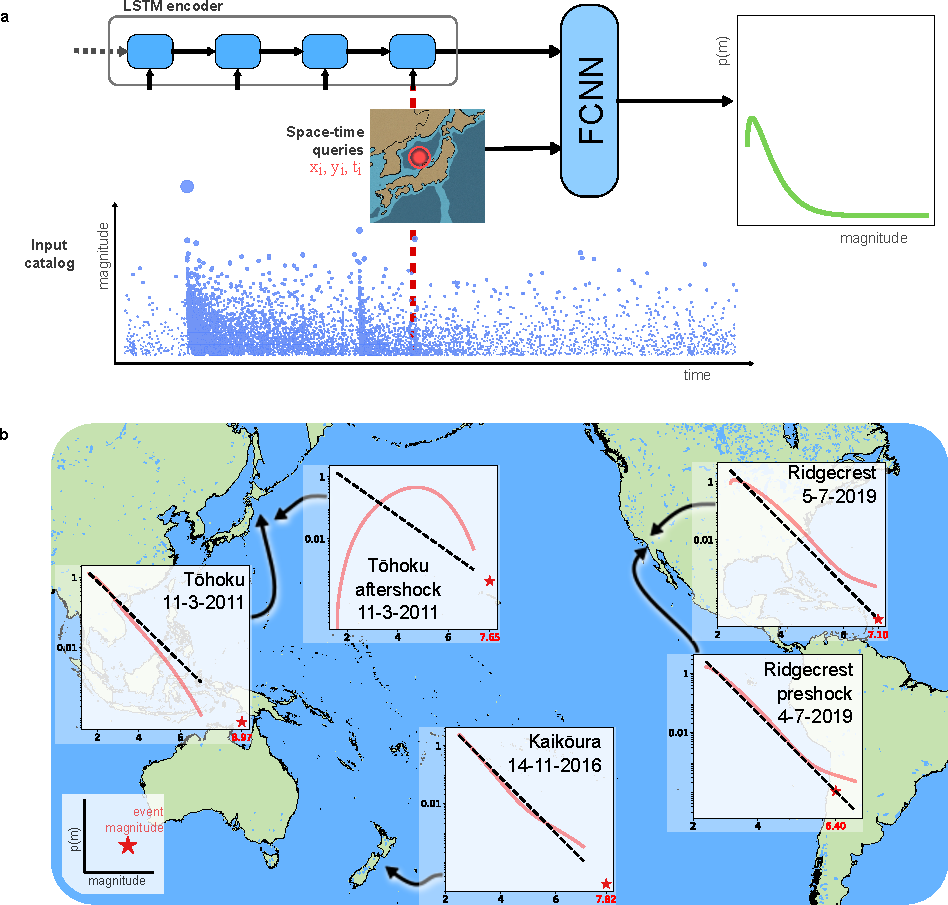
\includegraphics[width=1\textwidth]{figures/intro_fig.pdf}
	\caption{
 Caption.
}
\label{fig:intro_fig}
\end{figure}



\section{Results} \label{sec:results}

Focusing on existing events within the catalog due to our model's requirement for labeled data, our analysis utilizes the space-time coordinates of earthquakes as input. This necessitates excluding queries about arbitrary spatiotemporal points during training and evaluation, as these processes require knowledge of the true magnitude for each event at its specific location and time. Consequently, the raw output for our analysis consists of the model-generated PDFs of possible magnitudes for each event's time and location. Figure \ref{fig:architecture}b showcases PDFs produced by our model, $p_{\textbf{x}_i, t_i}(m)$, for 100 randomly sampled event times and locations from the test set. Included as a baseline is the stationary GR predictor trained on the training set, representing its potential operational use (e.g., Tsuruoka et al., 2012). A clear trend emerges: PDFs predicted for higher-magnitude events (warm colors) exhibit a greater skew towards higher magnitudes compared to those for lower-magnitude events (cooler colors). Figure \ref{fig:output_pdfs}a further highlights this trend by displaying a selection of model-generated PDFs alongside the corresponding likelihood of retrieving the true magnitude at the time and location each PDF was estimated for, denoted by a [color] circle.

Figure \ref{fig:output_pdfs}b focuses solely on the likelihood scores for retrieving the true magnitude, omitting the underlying PDFs used for their estimation. Additionally, it compares these scores against those generated by various benchmark models. Notably, our model demonstrates an advantage for most events exceeding magnitude $\sim 3$, while slightly under performing for lower-magnitude events. However, the overall mean log-likelihood (LL) score defined in \ref{eq:loss_function} (evaluated using the model-specific $p_{\textbf{x}_i, t_i}(\cdot)$ for each event) reveals a consistent advantage for our model across all datasets examined as summarized in \ref{tab:mean_ll}, where our model consistently obtains the lowest minus mean LL score in each column.



The information gain achieved by our model for each event can be quantified by the difference in log-likelihood (LL) between our model's prediction and the baseline GR predictor:
\begin{equation}
    \Delta LL = \log{p_{\pmb{x_i}, t_i}^{(model)}(m_i)} - \log{p^{(GR)}(m_i)}
    \label{eq:information_gain}
\end{equation}
This equation measures the number of bits of information gained by using our model compared to the GR benchmark. Analyzing this quantity per event across the entire test set reveals patterns in where our model achieves its advantage. \ref{fig:likelihood_over_time}a shows the Hauksson data test set event magnitudes at their occurrence times, colored according to the information gain. This time-domain representation allows us to track the cumulative information gain, calculated over the entire test set and displayed as a gray dashed line in the figure. The predominantly increasing trend in cumulative information gain suggests that our model is consistently advantageous as opposed to a concentrated advantage in specific periods. Notably, for the Hauksson data set, the most rapid information gain occurs during the aftershocks of the two Ridgecrest earthquakes. Surprisingly, even the pre-shock and main shock events demonstrate positive information gains over the GR benchmark, with values of $0.5$ and $1.4$ bits, respectively, though these events are typically considered completely unpredictable. This observation leads to a significant corollary: at least some portion of the information gain likely originates from a physical precursory signal. This point will be further elaborated upon in the discussion section.
\newline
The observed increase in information gain persists throughout the entire test set for all regions examined in this study. This includes regions previously analyzed by (Ogata et al. SRL 2018), where no information gain was detected using the method employed at the time. Further analysis of \ref{fig:likelihood_over_time} applied to other regions is presented in the supplementary material.
\newline
While the information gain observed in pre- and mainshocks presented above is encouraging, a potential concern might arise regarding the aftershocks: could their information gain be an artifact of fitting to the temporal incompleteness of the catalog (cite somethong?)? To address this, we factor out this potential bias by recalculating the likelihood score of each event, $p(m_i)$ , conditioned on the magnitude exceeding a threshold, $\Tilde{m}$:

\begin{equation}
    p \left( m \vert m_i > \Tilde{m} \right) = \frac{p_{\pmb{x}_i, t_i}(m)} {\int_{\Tilde{m}}^{\infty} p(m') ,dm'}
    \label{eq:conditioned_likelihood}
\end{equation}

For our analysis, we set $\Tilde{m} = m_c(t)$, determined dynamically using the maximum curvature method (Weimer and Weiss, 2000) within a window of 150 past and 150 future events. The resulting temporal incompleteness over time is displayed in \ref{fig:likelihood_over_time}b.
Crucially, \ref{fig:likelihood_over_time}b also presents the magnitudes of the Ridgecrest sequence at their origin times, colored by the information gain of our model over the GR benchmark, both conditioned on values above $m_c(t)$ as in \ref{eq:conditioned_likelihood}. This figure clearly demonstrates that even after accounting for temporal incompleteness, the information gain achieved by our model remains an increasing function throughout the test set. The mean score of the test set for the conditioned results are shown in [[]] which displays an outpreformance for our model with this metric as well. This finding underscores the ability of our model to capture true physical features beyond mere measurement artifacts.


[TODO: should I keep of remove the metrics for the causality defying metrics (present events) that beat the model in the ROC? this affects how the rest of this chapter will be written]




\begin{figure}[h!]
    \centering
    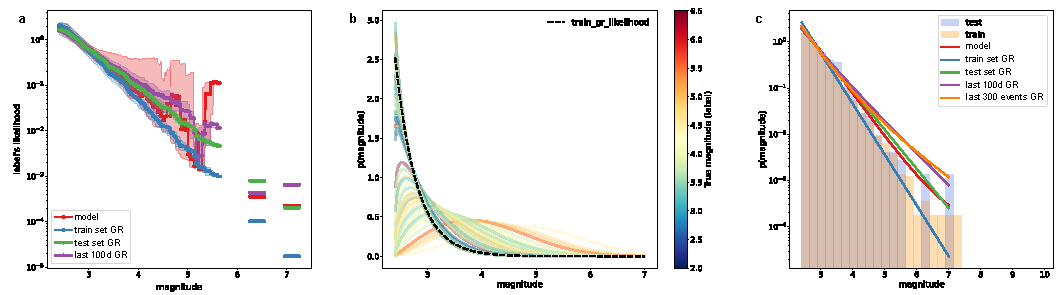
\includegraphics[width=1\textwidth]{figures/raw_results_hauksson.pdf}
    \caption{
        Caption.
    }
    \label{fig:architecture}
\end{figure}


\begin{figure}[h!]
    \centering
    \includegraphics[width=1\textwidth]{figures/info_over_time_hauksson.pdf}
    \caption{
        Caption.
    }
    \label{fig:architecture}
\end{figure}


\begin{figure}[h!]
    \centering
    \fbox{
        \rule{1\textwidth}{0pt}\rule{0pt}{8ex}
        FIGURE OF SPATIAL DISTRIBUTION OF GAIN.
    }
    \caption{
        Caption.
    }
    \label{fig:architecture}
\end{figure}

\begin{figure}[h!]
    \centering
    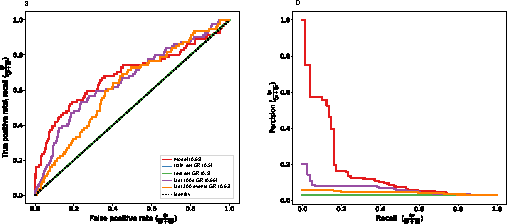
\includegraphics[width=0.4\textwidth]{figures/ROC_PR_hauksson.pdf}
    \caption{
        Caption.
    }
    \label{fig:architecture}
\end{figure}









% There are two bibliographies in Nature papers. One for the main text, and one for the Methods and Extended Data sections. The numbering is sequential, meaning that the reference section for the Methods and Extended Data section starts after the last number from the main reference section. References should not appear in both sections. Any reference used in Methods or Extended Data that also appears in the main bibliography should *only* appear in the main bibliography.
\let\oldbibliography\thebibliography
\renewcommand{\thebibliography}[1]{%
  \oldbibliography{#1}%
  \setlength{\itemsep}{10pt}%
}
% \bibliography{bibliography}
% \bibliography{bib-article.bib}
\newpage
\bibliography{Magnitude_prediction_paper}

\let\oldthebibliography=\thebibliography
\let\oldendthebibliography=\endthebibliography
\renewenvironment{thebibliography}[1]{
    \oldthebibliography{#1}
    % The number here (34 is an example) is the number of references in the main bibliography, and thus defines the starting number of the first reference in the Methods and Extended Data bibliography.
    \setcounter{enumiv}{34}
}{\oldendthebibliography}

% Figure legends appear after the text, not placed in the text. Do not include the actual image files in the article. Images are submitted as separate files. During the first submission to the journal, you can include the images in the article file for readability, but if you pass the reviews, they will want the images removed from the main article.
\newpage
\unnumbered

\unnumbered
\section{Methods}
\subsection{AI Model}
\textbf{Grey's Note} \textit{My understanding is that you can write the methods section just how you would a normal methods section for a normal scientific article.}


\section*{Data Availability}
This is a required section. Guidelines for data availability: \url{https://www.nature.com/documents/nr-data-availability-statements-data-citations.pdf}.

\section*{Code Availability}
\textbf{Grey's Note} \textit{This is a required section. If your article is about AI or ML, the editor will ask you to make the weights of a trained model available.}


\newpage
\renewcommand\refname{Methods References}
\begin{thebibliography}{10}

\bibitem{kratzert2019towards}
Frederik Kratzert, Daniel Klotz, Guy Shalev, G{\"u}nter Klambauer, Sepp
  Hochreiter, and Grey~S Nearing.
\newblock Towards learning universal, regional, and local hydrological
  behaviors via machine learning applied to large-sample datasets.
\newblock {\em Hydrology and Earth System Sciences}, 23(12):5089--5110, 2019.

\bibitem{klotz2022uncertainty}
Daniel Klotz, Frederik Kratzert, Martin Gauch, Alden~K Sampson, Johannes
  Brandstetter, G{\"u}nter Klambauer, Sepp Hochreiter, and Grey~S Nearing.
\newblock Uncertainty estimation with deep learning for rainfall--runoff
  modeling.
\newblock {\em Hydrology and Earth System Sciences}, 26(6):1673--1693, 2022.

\bibitem{twb2023gdp}
IBRD-IDA.
\newblock {The World Bank Data: Current US\$}.
\newblock https://data.worldbank.org/indicator/NY.GDP.MKTP.CD, 2023.
\newblock Accessed: 2023-06-04.

\end{thebibliography}


\newpage
\section*{Acknowledgements}
Acknowledgements should be brief, and should not include thanks to anonymous referees and editors, inessential words, or effusive comments. A person can be thanked for assistance, not “excellent” assistance, or for comments, not “insightful” comments, for example. Acknowledgements can contain grant and contribution numbers.

\section*{Author Contributions}
Author Contributions: Authors are required to include a statement to specify the contributions of each co-author. The statement can be up to several sentences long, describing the tasks of individual authors referred to by their initials. See the authorship policy page for further explanation and examples.


\section*{Author Information}
\textbf{Grey's Note} \textit{Two things are required in this Author Information section: (1) A statement about competing interests. I have no advice about what constitutes a competing interest, you will have to read about it and make your own decision. (2) A clear statement about who to contact with question about the paper. An example is below.}

The authors declare no competing interests. Please contact either the first author (Grey Nearing; \href{mailto:nearing@google.com}{nearing@google.com}) or Avinatan Hassidim; \href{mailto:avinatan@google.com}{avinatan@google.com}) for correspondence and requests, including questions regarding reprints and permissions.


\newpage
\section*{Extended Data}
\textbf{Grey's Note} \textit{You get up to 10 items in the Extended Data section. All Tables and Figures should be enumerated as "Extended Data Figure 1", "Extended Data Table 1", etc. These must also be referenced the same way in the text. Extended Data tables and figures may be referenced in the main article and/or in the Methods section. I am doing the in-text references to these ED items manually, instead of trying to override the table numbering schemed in Latex. Please update this template to automate that process if you feel like doing that.}

\textit{You can use Latex formatting for tables, but the journal will eventually require that your tables be submitted as images. Yes, this also struck me as unusual.}

\textit{Each ED figure should be on a separate page.}

\textit{Finally, this note is here in the ED section, but in your paper, the ED section should not have any text except figure and table captions/legends.}

\end{document}
